\documentclass[11pt,a4paper]{article}

\usepackage[utf8x]{inputenc}
\usepackage[T1]{fontenc}

\usepackage{pdfpages}
\usepackage{palatino}
\usepackage{enumitem}
\usepackage{outlines} %support nested list
\usepackage{float}
\usepackage{framed}

\usepackage{desclist}

\setlist[itemize]{topsep=3pt,after=\vspace{.5\baselineskip}}
\usepackage[left=3cm,right=3cm,top=3cm,bottom=3cm]{geometry}
\setlength{\parskip}{2mm}


\def\blurb{\textsc{Université catholique de Louvain\\
  École polytechnique de Louvain\\
  Pôle d'ingénierie informatique}}
\def\clap#1{\hbox to 0pt{\hss #1\hss}}%
\def\ligne#1{%
  \hbox to \hsize{%
    \vbox{\centering #1}}}%
\def\haut#1#2#3{%
  \hbox to \hsize{%
    \rlap{\vtop{\raggedright #1}}%
    \hss
    \clap{\vbox{\vfill\centering #2\vfill}}%
    \hss
    \llap{\vtop{\raggedleft #3}}}}%
\begin{document}

\begin{titlepage}
\thispagestyle{empty}\vbox to 1\vsize{%
  \vss
  \vbox to 1\vsize{%
    \haut{\raisebox{-5mm}{
\includegraphics[width=2.5cm]{img/logo_ucl.pdf}}}{\blurb}{\raisebox{-5mm}{
\includegraphics[scale=0.20]{img/ingi_logo.png}}}
    \vfill
    \ligne{\Huge \textbf{\textsc{LINGI2251}}}
     \vspace{5mm}
    \ligne{\huge \textbf{\textsc{Software Engineering: Development Methods}}}
     \vspace{15mm}
    \ligne{\Large \textbf{\textsc{Assignment 1}}}
    \vspace{5mm}
    \ligne{\large{\textsc{16 march 2016}}}
    \vfill
    \vspace{5mm}
    \ligne{%
         \textsc{Alexandre Hauet\\Tanguy Vaessen} 
      }
      \vspace{5mm}
    }%
  \vss
  }
\end{titlepage}

%\tableofcontents


\section{Requirements adjustment}
\begin{itemize}
	\item Gas pump can either send a message when the transaction is over with the number of gallons purchased (from requirement 1) or it can send 2 messages: one when the transaction is over with no parameters and one to indicates the amount of gas and the amount of dollars for the transaction.
We chose the second option because the system might want to know the current amount of gas and dollar during the transaction and not only at the end. This is possible with the 2 separates messages.
	\item In the requirements, the local businesses have billing accounts set up to receive a monthly bill, instead of paying at the time of purchase. And customers can pay directly or have a billing accounts. 
We think, there is a omissions the local businesses can also pay directly and don't need systematically a billing account.
	\item The term Gas Station Control System (GSCS) can be ambiguous. It is used a lot of times in the requirements, and some times it refers to a kind of interface. For us, the term GSCS refers to the whole system.
\end{itemize}


\section{Interfaces}

\paragraph{Note:}  
\begin{itemize}
\item IN = message received by our GSCS system from the entity
\item OUT = message send by our GSCS to the entity
\end{itemize}


\subsection{Customers (external entity)}
\subsection{Cashier (external entity)}
\subsection{Cashier's interface}
\begin{itemize}
\item IN : 
	\begin{itemize}
		\item cashier\_input (input): the cashier has input the given input (for example that the payment is completed or that the payment will be made by monthly bill). \\
		\textbf{input} : numeric, option, ...
	\end{itemize}
\item OUT :
	\begin{itemize}
		\item message(string): message to be display at the cashier’s interface. \\
		\textbf{string} : unknow format (for example ask the cashier for the billing account number).
	\end{itemize}
\end{itemize}


\subsection{Credit card reader}
\begin{itemize}
\item IN : 
	\begin{itemize}
		\item card\_ readed(credit\_ card\_ number): a card has been read with the given credit card number. \\
		\textbf{credit\_ card\_ number} : a valid credit card number.
		\item invalid\_ card\_ read() : an invalid card has been read.
	\end{itemize}
\end{itemize}

\subsection{Credit card system}
\begin{itemize}
\item OUT : 
	\begin{itemize}
		\item  do\_ purchase(credit\_ card\_ number, amount) : ask the credit card system to proceed the payment with the given credit card number for the given amount. \\
		\textbf{credit\_ card\_ number} : a valid credit card number. \\
		\textbf{amount} : a positive real number between 0 and 10000.
	\end{itemize}
\end{itemize}

\subsection{Gas pump}
\begin{itemize}
\item IN : 
	\begin{itemize}
		\item  customer\_ has\_ finished\_ dispensing\_ gas(): inform the GS CS that the customer has finished dispensing gas.
		\item  current\_ values(amount\_ of\_ gas, dollar\_ amount): give information about the current amount of gas and the current amount of dollars taken by the customer. \\
		\textbf{amount\_ of\_ gas} : real positive number. \\
		\textbf{dollar\_ amount} : a positive real number between 0 and 999,99.
	\end{itemize}
\end{itemize}

\subsection{Gas pump interface }
\begin{itemize}
\item IN : 
	\begin{itemize}
		\item  option\_choice(option): the user has selected the option \textit{option} (for example the chosen payment method). \\
		\textbf{option} : unknow format.
	\end{itemize}
\item OUT : 
	\begin{itemize}
		\item  message(string): message to be displayed to the customer (for example choose a payment method). \\
		\textbf{string} : unknow format.
	\end{itemize}
\end{itemize}




\section{State of the system}

\begin{outline}
	\1 Payment type: the customer can choose to pay directly or with a monthly bill. This is represented in this state value.
		\2 Data type : Enumeration
		\2 Data range: DirectPayment, MonthlyBill
	\1 Payment method: this state value records the payment method that the user has chosen.
		\2 Data type : Enumeration
		\2 Data range: it can be either Cash, CreditCard.
	\1 Gallons of fuel: The number of gallons of fuel that the current customer has already took from the pump.
		\2 Data type : Real number
		\2 Data range: [0, x] where x is the max capacity of the tank
	\1 Dollar amount: The amount that the customer has to pay 
		\2 Data type : Real number
		\2 Data range:  [0, 999.99]
	\1 Credit card number: if the customer has chosen to pay with credit card, the credit card number will be stored in this variable.
		\2 Data type : Credit card number
		\2 Data range: --
	\1 Payment status: this variable will state if the customer has done the payment or not.
		\2 Data type : boolean
		\2 Data range: [True, False]
	\1 Billing account number: the account number to which the bill must be send at the end of the month.
		\2 Data type : Account number
		\2 Data range: --
\end{outline}

\section{Data-flow diagram}
%The data-flow diagram is drawed in Figure \ref{fig:dataflow} on page \pageref{fig:dataflow}.

\begin{figure}[H]
 \centering
 \includegraphics[width=\textwidth]{../data-flow-diagram.png} 
 \caption{Data-flow diagram}
 \label{fig:dataflow}
\end{figure}


\section{Class diagram for the system}

%The class diagram is drawed in Figure \ref{fig:class} on page \pageref{fig:class}.


\subsection*{Sequence diagrams for the following scenarios:}
\begin{enumerate}
	\item A customer successfully purchases gas and charges it on a monthly bil: drawed in Figure \ref{fig:sequence1} on page \pageref{fig:sequence1}.
	\item A customer purchases gas and attempts to pay by credit card but his card is refused. He then pays by cash to the cashier: drawed in Figure \ref{fig:sequence2} on page \pageref{fig:sequence2}.
	\item The cashier successfully processes a monthly payment by credit card: drawed in Figure \ref{fig:sequence3} on page \pageref{fig:sequence3}.
\end{enumerate}

\begin{figure}[H]
 \centering
 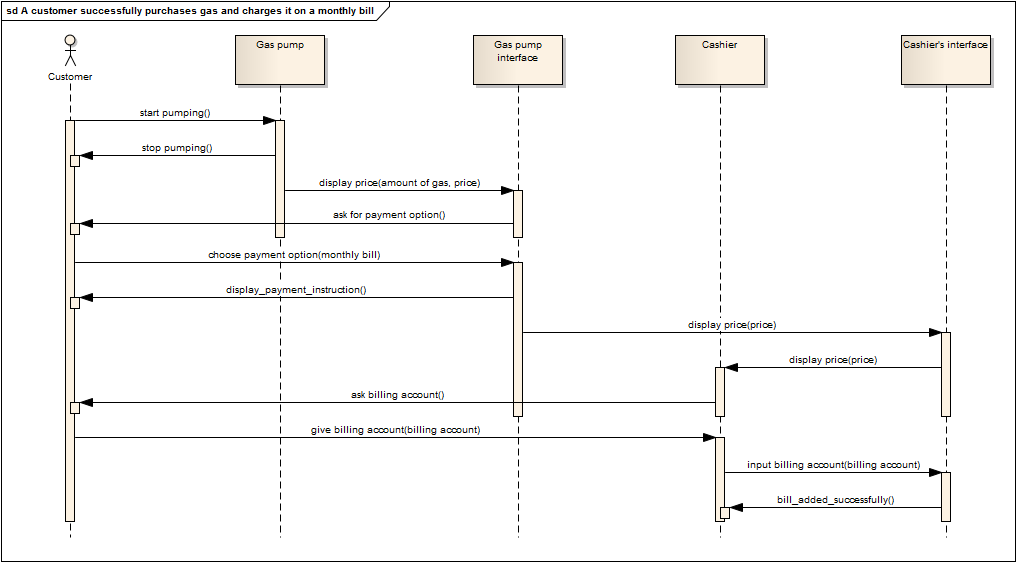
\includegraphics[width=\textwidth]{../sequence1.png} 
 \caption{A customer successfully purchases gas and charges it on a monthly bil.}
 \label{fig:sequence1}
\end{figure}

\begin{figure}[H]
 \centering
 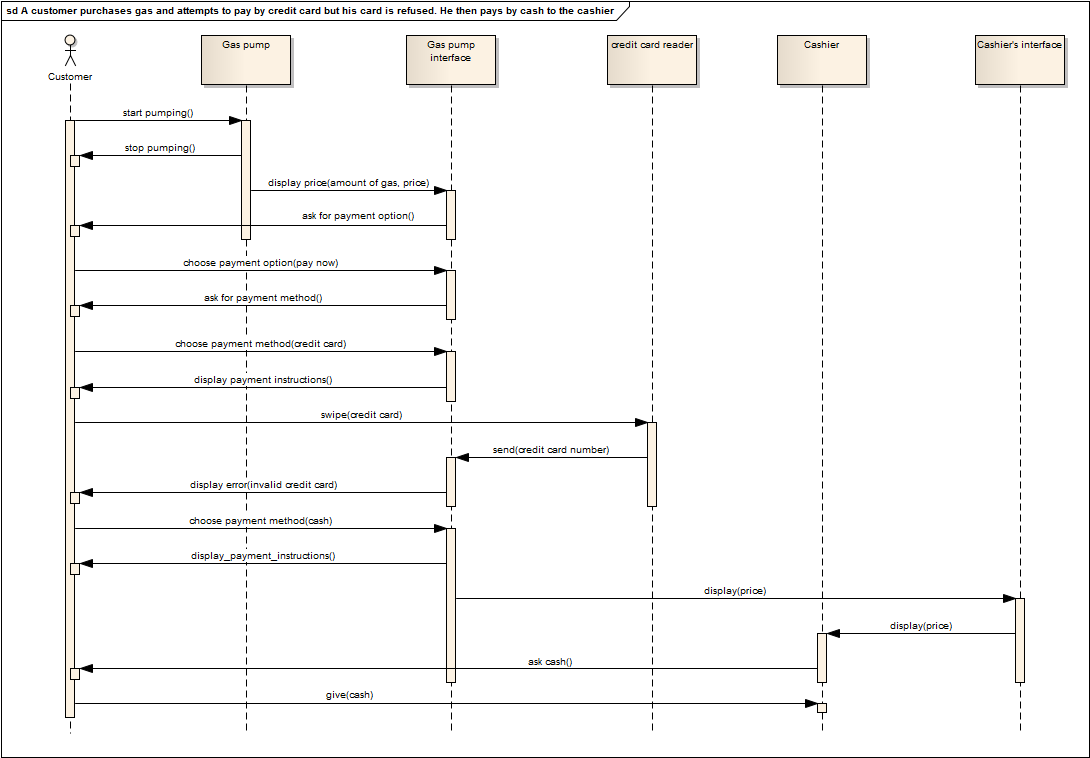
\includegraphics[width=\textwidth]{../sequence2.png} 
 \caption{A customer purchases gas and attempts to pay by credit card but his card is refused. He then pays by cash to the cashier.}
 \label{fig:sequence2}
\end{figure}

\begin{figure}[H]
 \centering
 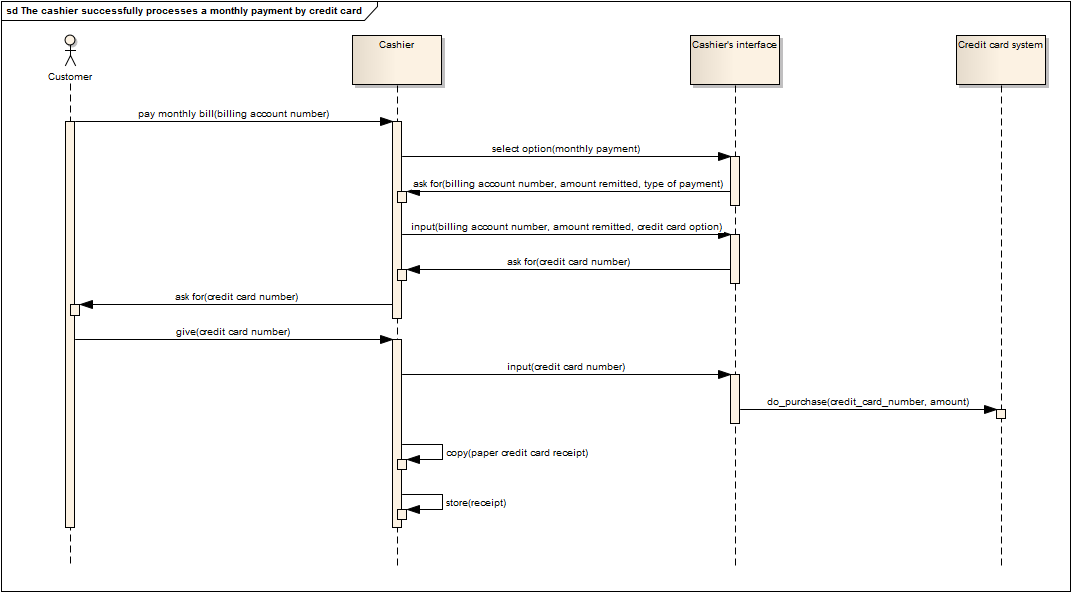
\includegraphics[width=\textwidth]{../sequence3.png} 
 \caption{The cashier successfully processes a monthly payment by credit card.}
 \label{fig:sequence3}
\end{figure}


\section{State diagrams}


\begin{enumerate}
	\item Gas pump interface's state diagram: drawed in Figure \ref{fig:state1} on page \pageref{fig:state1}.
	\item Cashier's interface's state diagram: drawed in Figure \ref{fig:state2} on page \pageref{fig:state2}.
\end{enumerate}

\begin{figure}[H]
 \centering
 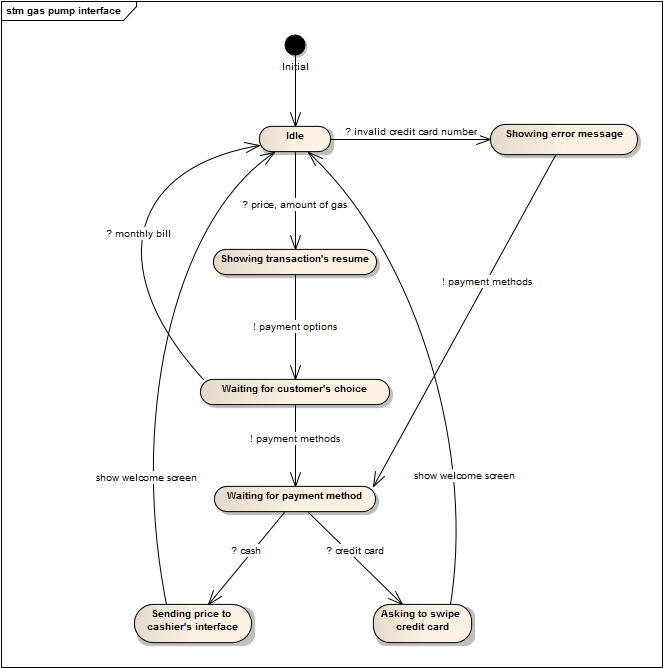
\includegraphics[width=\textwidth]{../state-diagram-gas-pump-interface.png} 
 \caption{State diagram - Gas pump interface}
 \label{fig:state1}
\end{figure}

\begin{figure}[H]
 \centering
 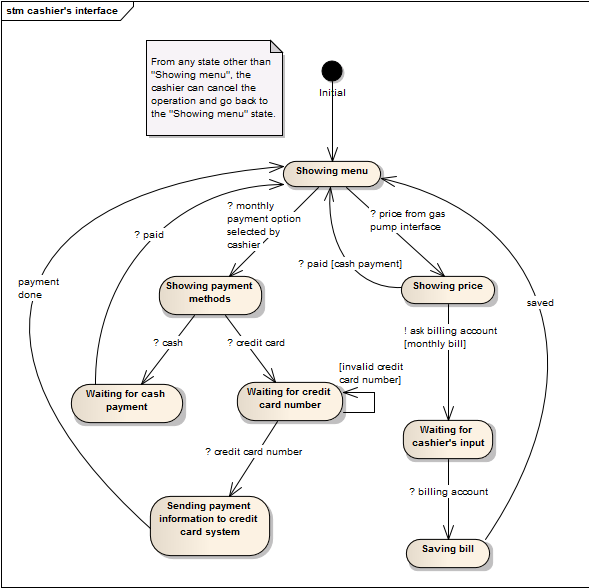
\includegraphics[width=\textwidth]{../state-diagram-cashier-interface.png} 
 \caption{State diagram - Cashier's interface}
 \label{fig:state2}
\end{figure}



\end{document}
